% Generated by pysimcount.pfseeds -- do not edit; regenerate instead.
% figure: B-order6-by-formula -- Every order-6 formula at measured r; median over seeds [1, 2, 3, 4, 5, 6, 7, 8, 9, 10], bars = min..max
% metric=cnot gatebase=cz merged
% seed 1: git_commit=01d3c275ceae2840002bd1aaea68f59b987c4975 git_dirty=False
% seed 2: git_commit=01d3c275ceae2840002bd1aaea68f59b987c4975 git_dirty=False
% seed 3: git_commit=01d3c275ceae2840002bd1aaea68f59b987c4975 git_dirty=False
% seed 4: git_commit=01d3c275ceae2840002bd1aaea68f59b987c4975 git_dirty=False
% seed 5: git_commit=01d3c275ceae2840002bd1aaea68f59b987c4975 git_dirty=False
% seed 6: git_commit=01d3c275ceae2840002bd1aaea68f59b987c4975 git_dirty=False
% seed 7: git_commit=01d3c275ceae2840002bd1aaea68f59b987c4975 git_dirty=False
% seed 8: git_commit=01d3c275ceae2840002bd1aaea68f59b987c4975 git_dirty=False
% seed 9: git_commit=01d3c275ceae2840002bd1aaea68f59b987c4975 git_dirty=False
% seed 10: git_commit=01d3c275ceae2840002bd1aaea68f59b987c4975 git_dirty=False
% derived: B-order6-by-formula.tex restyled by pysimcount.figuniform: extrapolated points (r from power-law fit) drawn in their series' measured style, style-key legend entries removed; extrapolated n = [13, 20]; source_sha256=f79ab8e142953637d9346bf5eab91525b0bd099d8f3d8bf6a4671f3d0e65b386
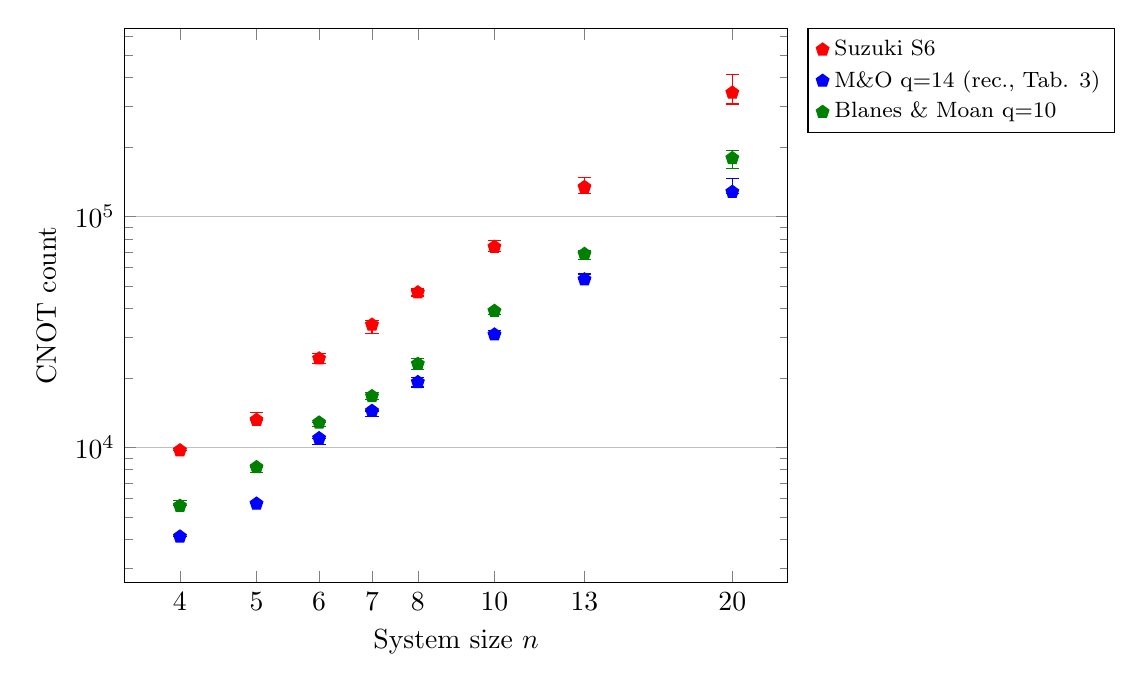
\begin{tikzpicture}
  \begin{loglogaxis}[
    width=10cm,
    xlabel={System size $n$},
    ylabel={CNOT count},
    xtick={4,5,6,7,8,10,13,20},
    xticklabels={4,5,6,7,8,10,13,20},
    ymajorgrids=true,
    legend pos=outer north east,
    legend cell align=left,
    legend style={font=\footnotesize},
  ]
    \addplot[only marks, red, mark=pentagon*, mark size=2.4pt, mark options={solid, fill=red}, error bars/.cd, y dir=both, y explicit, error bar style={red}] coordinates {
      (4,9696) += (0,0) -= (0,0)
      (5,13130) += (0,1010) -= (0,0)
      (6,24240) += (0,1212) -= (0,1212)
      (7,33936) += (0,1414) -= (0,2828)
      (8,46864) += (0,1616) -= (0,1616)
      (10,73730) += (0,5050) -= (0,3030)
    };
    \addlegendentry{Suzuki S6}
    \addplot[only marks, red, mark=pentagon*, mark size=2.4pt, mark options={solid, fill=red}, forget plot, error bars/.cd, y dir=both, y explicit, error bar style={red}] coordinates {
      (13,133926) += (0,13130) -= (0,7878)
      (20,343400) += (0,68680) -= (0,36360)
    };
    \addplot[only marks, blue, mark=pentagon*, mark size=2.4pt, mark options={solid, fill=blue}, error bars/.cd, y dir=both, y explicit, error bar style={blue}] coordinates {
      (4,4104) += (0,0) -= (0,0)
      (5,5700) += (0,0) -= (0,0)
      (6,10944) += (0,0) -= (0,684)
      (7,14364) += (0,0) -= (0,798)
      (8,19152) += (0,912) -= (0,912)
      (10,30780) += (0,1140) -= (0,0)
    };
    \addlegendentry{M\&O q=14 (rec., Tab. 3)}
    \addplot[only marks, blue, mark=pentagon*, mark size=2.4pt, mark options={solid, fill=blue}, forget plot, error bars/.cd, y dir=both, y explicit, error bar style={blue}] coordinates {
      (13,53352) += (0,2964) -= (0,0)
      (20,127680) += (0,18240) -= (0,2280)
    };
    \addplot[only marks, green!50!black, mark=pentagon*, mark size=2.4pt, mark options={solid, fill=green!50!black}, error bars/.cd, y dir=both, y explicit, error bar style={green!50!black}] coordinates {
      (4,5576) += (0,328) -= (0,0)
      (5,8200) += (0,0) -= (0,410)
      (6,12792) += (0,0) -= (0,492)
      (7,16646) += (0,574) -= (0,574)
      (8,22960) += (0,1312) -= (0,1312)
      (10,38950) += (0,410) -= (0,1230)
    };
    \addlegendentry{Blanes \& Moan q=10}
    \addplot[only marks, green!50!black, mark=pentagon*, mark size=2.4pt, mark options={solid, fill=green!50!black}, forget plot, error bars/.cd, y dir=both, y explicit, error bar style={green!50!black}] coordinates {
      (13,68757) += (0,2665) -= (0,3731)
      (20,178760) += (0,14760) -= (0,18040)
    };
  \end{loglogaxis}
\end{tikzpicture}
